
Can you tell whether a coin is fair or bent, given the following independent coin toss results:
\begin{figure*}[h]
\centering
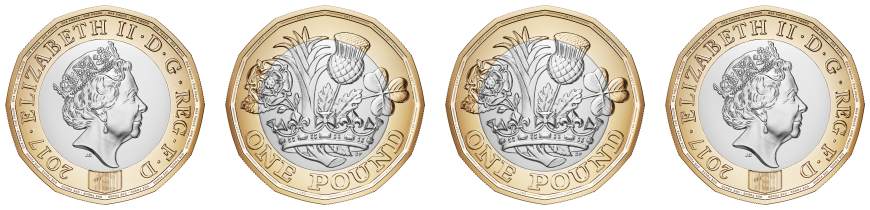
\includegraphics[width=0.4\linewidth]{Chapter1/coinflip.png}
\vspace{-1em}
\end{figure*}
\begin{center}
head, tail, tail, head.
\end{center}

Maybe you would say ``the coin is fair''.  But why, and how \emph{confident} you are in your answer? Furthermore, if I offered you a bet on the next outcome of a coin flip, at what odds would you take that bet?

A Bayesian statistician can easily answer all of the above questions by following Bayesian decision theory \citep{bishop:prml2006, berger:decision2013}. Before observing the coin flip results, he/she will first determine a \emph{prior belief} on whether the coin is bent or not. Usually this belief is represented by two probability values $P(\text{fair})$ and $P(\text{bent})$ that sum to one. 
%
Then he/she builds a conditional probability -- for example $P( \text{head} | \text{fair} )$ is the probability of the coin flip ``head'' given that the coin is fair -- to describe the \emph{likelihood} of a fair/bent coin given an observation. 
%
After observing some simulation outcomes, he/she will adjust his/her \emph{posterior belief} on the unknown properties of the coin using \emph{Bayes' rule} \citep{bayes:bayes_rule1763, laplace:theorie1820}:

\begin{equation}
P(\text{fair} | \text{coin flip results} ) = \frac{P( \text{coin flip results} | \text{fair}) P(\text{fair})}{ P(\text{coin flip results})}
\label{eq:intro_bayes_rule}
\end{equation}
where in our example, the conditional and marginal probabilities are calculated by simply following the sum rule and product rule of probability:
$$ P( \text{coin flip results} | A) = P( \text{head} | A) P( \text{tail} | A) P( \text{tail} | A) P( \text{head} | A), \quad A \in \{ \text{fair}, \text{bent} \} ,$$
$$ P( \text{coin flip results}) = P( \text{coin flip results} | \text{fair}) P(\text{fair}) + P( \text{coin flip results} | \text{bent}) P(\text{bent}) .$$

The Bayesian statistician can finally answer the question, by picking the one with the largest \emph{posterior probability}, i.e.~the coin is fair if 
$$P(\text{fair} | \text{coin flip results} ) > P(\text{bent} | \text{coin flip results} ),$$
or the coin is bent otherwise. Furthermore, he/she can tell us how confident he/she is, for example ``the posterior probability of the coin being fair is $60\%$, so I am not very confident when saying the coin is fair''. In general, by gathering more coin flip results (more than four simulation outcomes in this case), he/she continues adjusting the posterior belief for a fair/bent coin using Bayes' rule, and becomes more confident about the inferred answer. Having the inference result at hand, he/she can even predict the outcome of a future coin flip experiment, again with an uncertainty estimate, then decide whether he/she should accept the bet as well as the correct odds yielding a positive expected return.

The coin flip problem is just an elementary example of \emph{Bayesian inference}, and in general these principles of inference and decision making apply to many real-world tasks as well. Powered by the rules of probability, Bayesian methods allow us to infer the unknown factors given the observed data, quantify the confidence of the inferred results, and make predictions with calibrated uncertainty estimates that support decision making. Critically, \cite{cox:axioms1946} argued that, reasoning under probability rules is the \emph{only} way to perform coherent inference under uncertainty.\footnote{Also see chapters 1 and 2 in \cite{jaynes:book2003}.} So ideally, Bayesian methods should be applied to any situation where well-calibrated inferences need to be made from data. These include prediction tasks such as classifying cat and dog images, and decision making tasks like determining the next action for a robot.

Despite having many desirable theoretical properties, Bayesian methods are less widely used in many exciting applications of artificial intelligence, especially those powered by deep learning \citep{lecun:deeplearning2015, schmidhuber:deeplearning2015, goodfellow:deeplearning2016} such as the AlphaGo system \citep{silver:alphago2016, silver:alphagozero2017} that defeated human Go champion Ke Jie 3-0.\footnote{\url{https://en.wikipedia.org/wiki/AlphaGo_versus_Ke_Jie}}
%
Although the Bayesian approach maintains a posterior distribution of all possible settings of the unknown factors which is desirable, it also requires computing the marginal probability of the observations (in our example $P(\text{coin flip results})$) that involves evaluating \emph{all} possible settings of the neural network weights. Observing this, a deep learning practitioner might respond that ``it takes \emph{forever} to compute Bayes' rule for my task, so I'd better stick to a point estimate that minimises the training error.'' Two recent trends of deep learning applications make the situation even worse for Bayesian inference: 1) the neural networks employed are getting deeper and wider \citep{he:resnet2016, huang:stochastic_depth2016, huang:dense_net2017}, and 2) a typical dataset for deep learning tasks contains millions (if not billions) of instances \citep{deng:imagenet2009, abu:youtube8m2016}.

%

But still, uncertainty quantification is crucial to achieving better deep learning. First, deep learning models are often over-parameterised, and using a point estimate can easily lead to over-fitting and poor predictive performance. Second, as nowadays deep learning techniques are being incorporated into many systems affecting the quality of human life (e.g.~intelligent personal assistants, machine translation, even intelligence systems supporting autonomous driving and health care), it is crucial to make sure these systems know \emph{how confident the model is when performing decision making}. Also, uncertainty information is essential to solving the exploration-exploitation trade-off, which helps learn a better agent faster in reinforcement learning and robotics applications \citep{deisenroth:pilco2011, mcallister:data_efficientRL2016}. Furthermore, Bayesian methods are the gold standard approaches for data efficiency, which is crucial to build a better prediction system for tasks that usually don't have \emph{enough} labelled cases, and potentially present lots of missing values, e.g.~medical applications.  

Fortunately, if fast and accurate \emph{approximation} schemes could be applied to the quantities that a Bayesian statistician would like to compute, then he/she can still perform (approximate) Bayesian inference and quantify the model uncertainty accordingly. Hence the primal challenge for Bayesian inference today is to design fast and accurate \emph{approximate inference} algorithms for complex systems like neural networks and scale them to large datasets, which will be the main subject of the thesis. But before we delve into the development of such algorithms, in the rest of this introductory chapter I shall introduce the mathematical background for approximate inference, and identify fundamental research questions about this subject.


